% This file is the Latex source of the Big Data course project
% report. The project contributors are Ali Alavi, Rolf jagerman
% and Ken Tsay.
% The report is written by Ali Alavi, Rolf Jagerman.

%
\documentclass{llncs}
%

\usepackage{graphicx} % for importing images
\usepackage{caption}
\usepackage{subcaption} % for subfigures
\captionsetup{compatibility=false} % to make subfigures compatible with template

\usepackage{url} % for URL references
\usepackage{float} % helps with locating the 
\usepackage[T1]{fontenc}  % providing font encoding
% used for drawing the diagrams
%
\begin{document}
%
\mainmatter              % start of the contributions
\pretolerance=10000  % This avoids long lines
\pagestyle{headings}
%\hyphenation{}

%
\title{Automatic News Generation Based on Twitter}
%
\titlerunning{Automatic News Generation Based on Twitter}  % abbreviated title (for running head)
%                                     also used for the TOC unless
%                                     \toctitle is used
%
\author{Ali Alavi\inst{1} \and Rolf Jagerman\inst{1} \and
Tsay Kai-En\inst{1}}
%
\authorrunning{Ali Alavi, Rolf Jagerman and Tsay Kai-En} % abbreviated author list (for running head)
%
%
\institute{ETH Z\"urich, Z\"urich, Switzerland\\
\email{alavis@ethz.ch, \{rolfj, tsayk\}@student.ethz.ch}
}

\maketitle              % typeset the title of the contribution
%

\section{Introduction}
% todo
This report presents the current status of the project \textbf{Automatic News Generation Based on Twitter}, for \textbf{Big Data} course (code \textit{263-3010-00L}). This project tries to answer the following questions: 
\textit{Can we automatically generate news headlines based on public twitter posts? Can this method of news generation perform better than the available news agencies, in terms of speed, reliability and so on?}

We tackle this problem by taking the following steps:

\begin{enumerate}
	\item \textit{Data collection: }Gathering a large set of twitter posts and news headlines 
	\item \textit{Building a classifier: }Use the news headlines to train a classifier
	\item \textit{Labeling the tweets: }Label each tweet using the classifier we previously trained
\end{enumerate}

A big picture of the system is depicted in Figure ~\ref{fig:A big picture of the system}. In the rest of this report we will elaborate how we implement the solution in a scalalaby way on Spark. 

\begin{figure}[H]
	\centering
	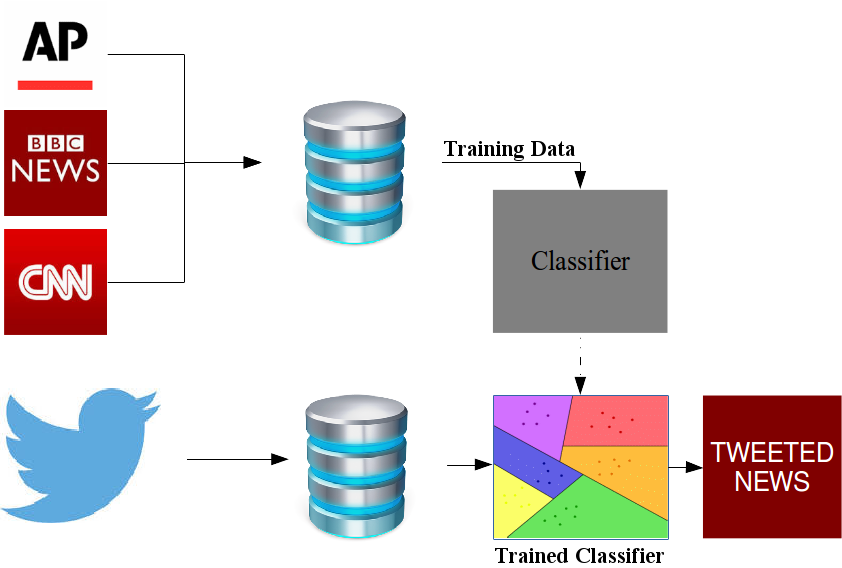
\includegraphics[width=0.8\textwidth]{images/bigpicture.png} 
	\caption{A big picture of the system}
	\label{fig:A big picture of the system}
\end{figure}



\section{Data model}
% todo
...


\section{Design of the system}
System architecture is depicted in Figure ~\ref{fig:Architecture design of the system}. The data storage component is on Amazon S3, and the data process platfrom is on Apache Spark. 

\begin{figure}[H]
	\centering
	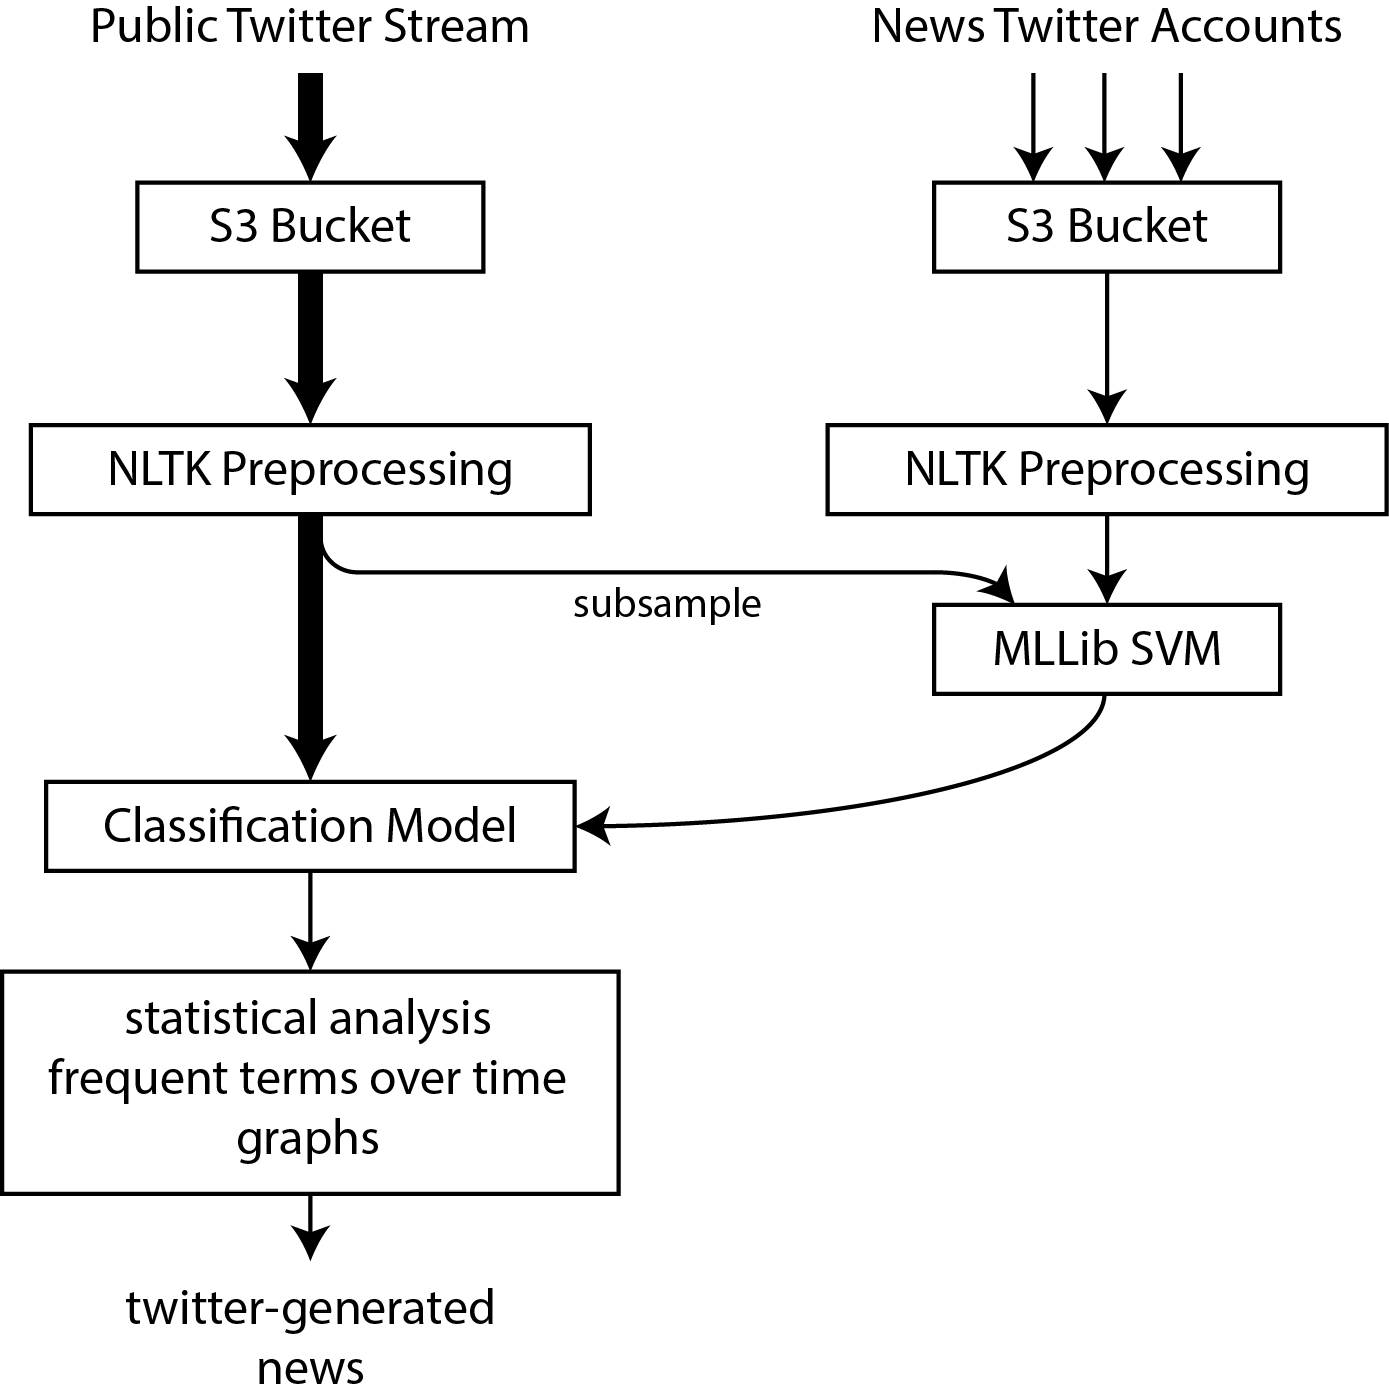
\includegraphics[width=0.8\textwidth]{images/system_arch.png} 
	\caption{Architecture design of the system}
	\label{fig:Architecture design of the system}
\end{figure}

\subsection{Data storage}
We stored around 600G of the twitter stream data on Amazon S3. Differ from previous work, we integrate the data collecting script with s3cmd tool, which is a command line tool and client for uploading, retrieving and managing data in Amazon S3~\cite{s3cmd}, and direct uploaded the twitter streamming data into S3 bucket. This benefit the whole system cause we can load the large training and prediction dataset via using S3 protocol into our Spark instance. 

\subsection{Data process platform}
We run Spark on top of Amazon Elastic Mapreduce(EMR). In the begining we were running Spark on Aamzon EC2, we create 


\subsection{Platform}

\section{Results}
% todo
...


\section{Future Work}
% todo
...




\bibliographystyle{plain}
\bibliography{report.bib}

\end{document}